\documentclass{standalone}

\usepackage{tikz}
\usetikzlibrary{calc}

\begin{document}
  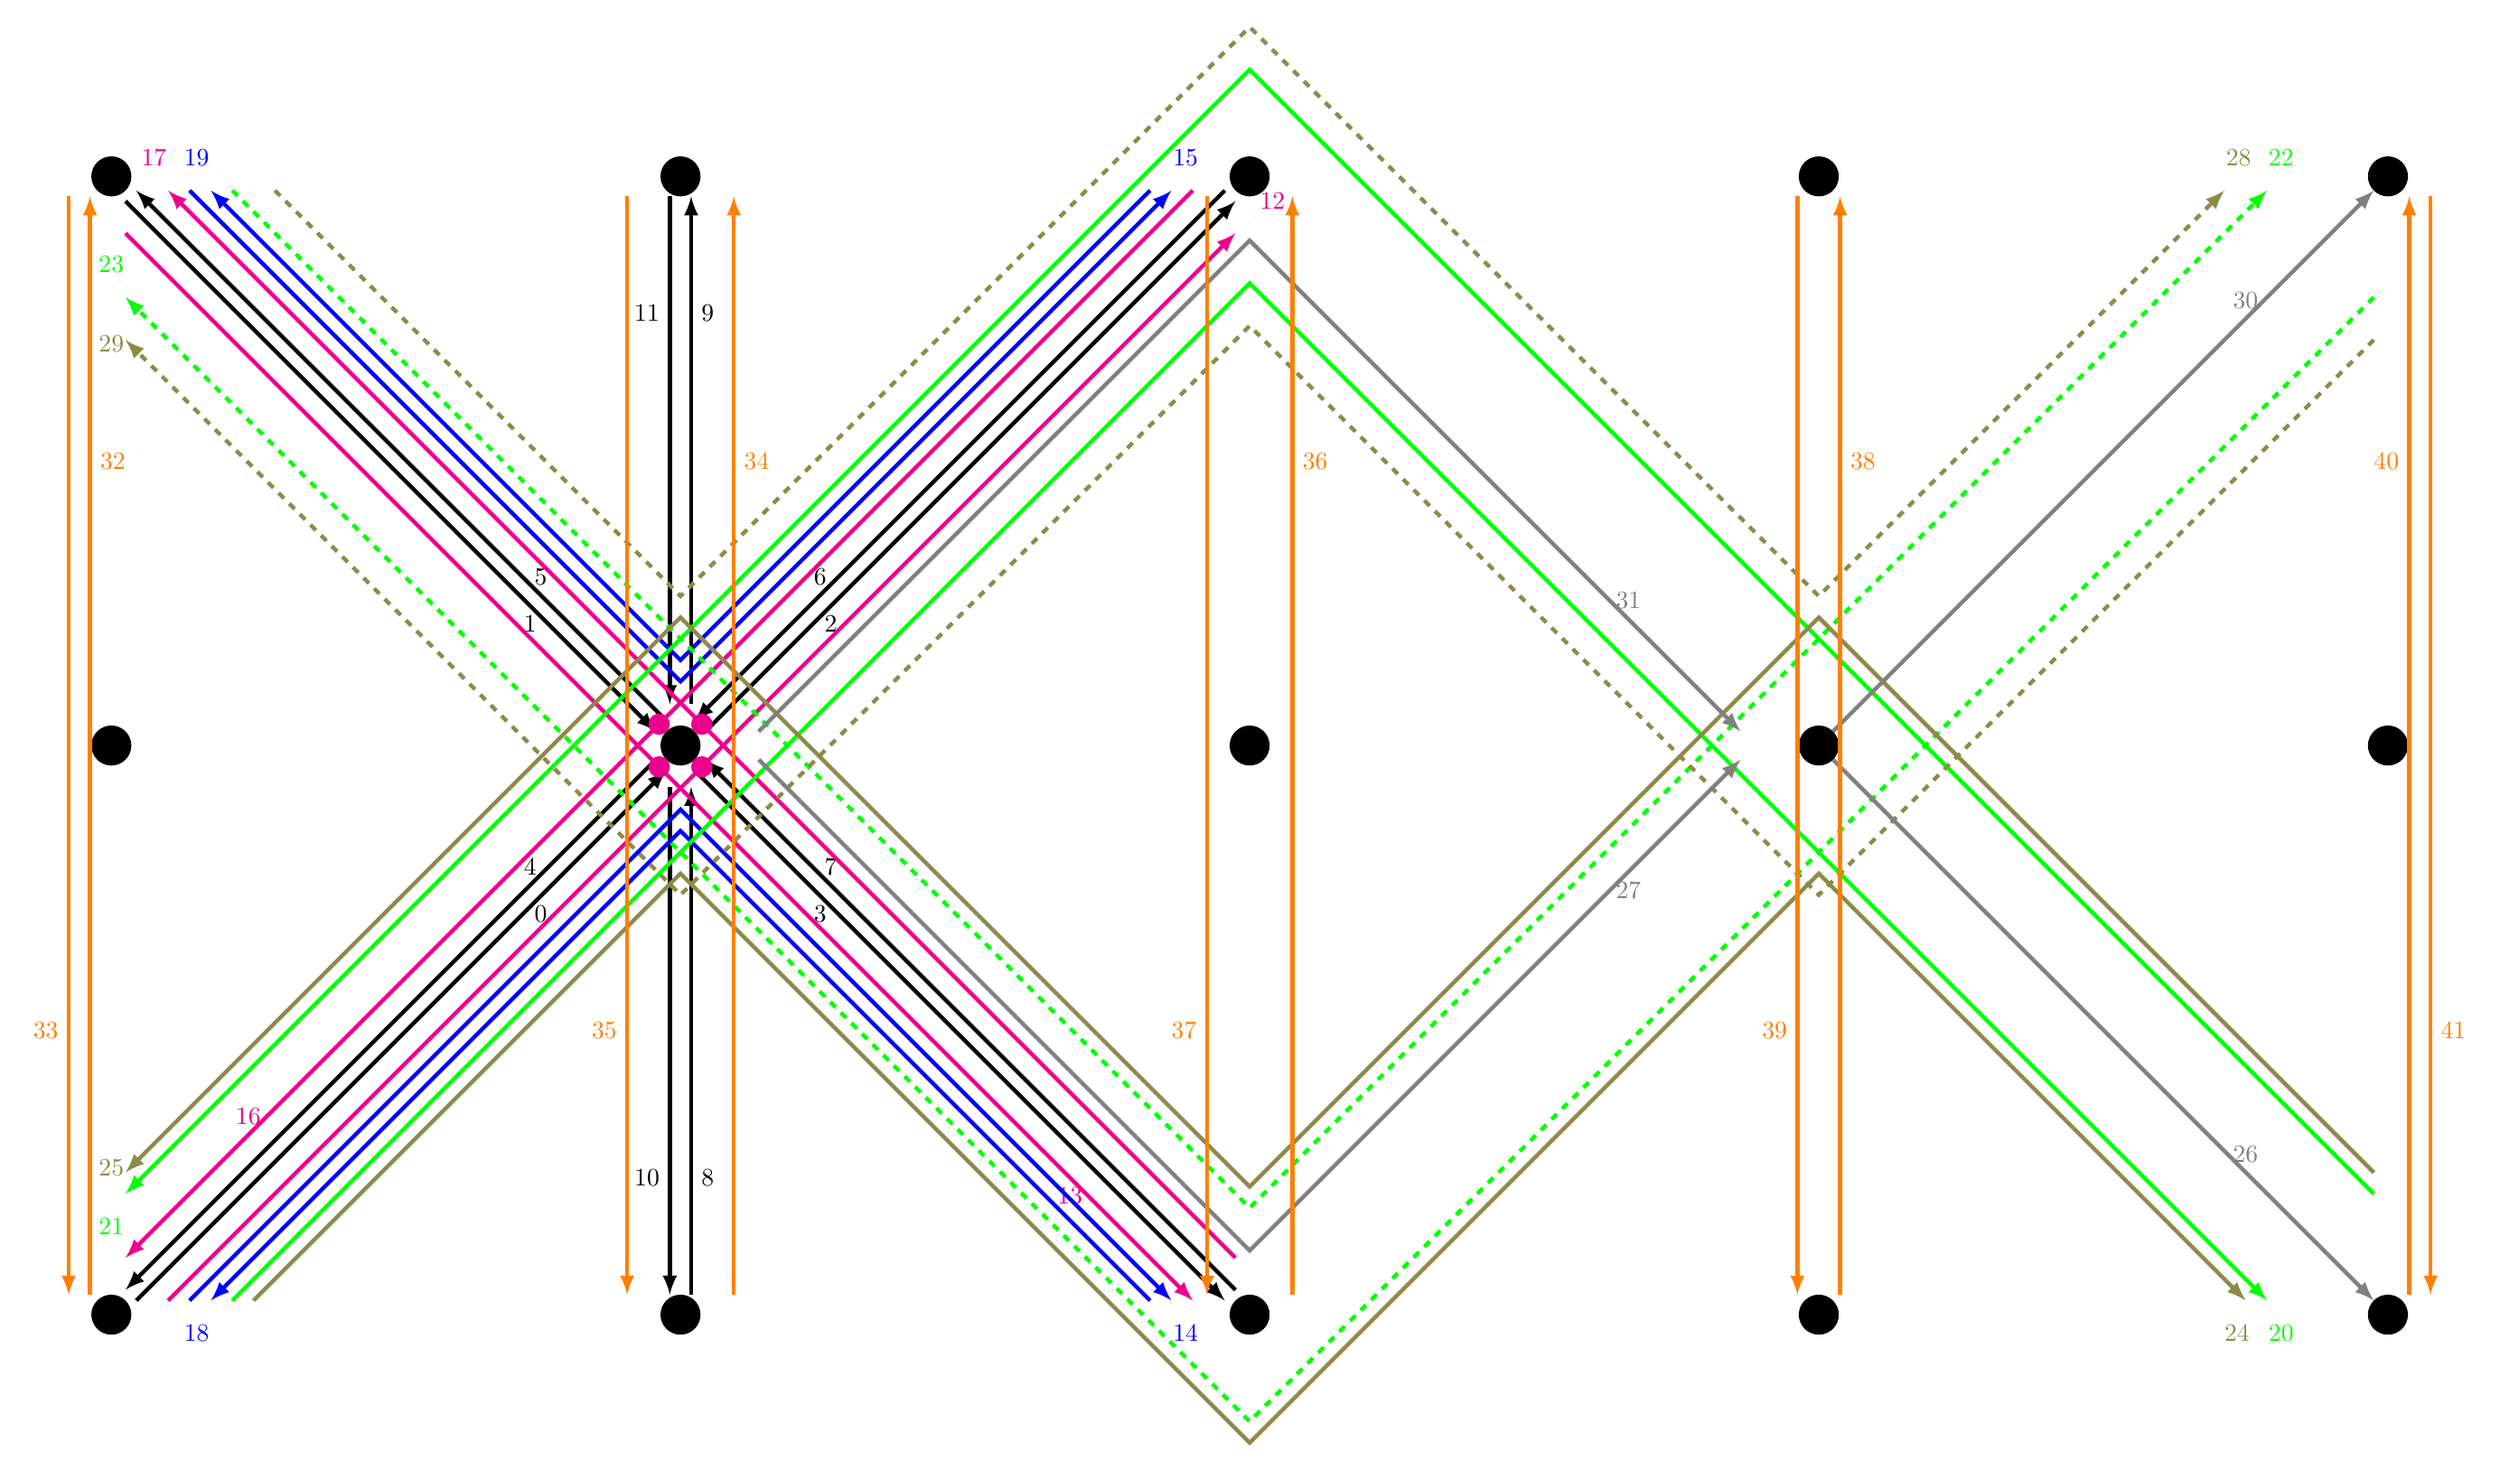
\begin{tikzpicture}
    \def\sep{0.15}

    \def\scalefact{8}
    \def\scalerad{\scalefact*1pt}

    \tikzset{
      ncbar/.style={
        to path=%
        ($(\tikztostart)!#1!90:(\tikztotarget)$)
        -- ($(\tikztotarget)!($(\tikztostart)!#1!90:(\tikztotarget)$)!90:(\tikztostart)$)
        (\tikztotarget) \tikztonodes
      },
      ncbar/.default=0.5cm,
    }

    \tikzset{%
      polyline/.style={%
        ultra thick, -latex, shorten <= \scalerad, shorten >= \scalerad}}

   % \draw[help lines,step=\scalefact] (0,0) grid ($(4*\scalefact ,2*\scalefact)$);
    \foreach \i in {0,1,2,3,4}
    \foreach \j in {0,1,2}{
      \coordinate (p\i\j) at ($(\scalefact*\i,\scalefact*\j)$);
      \fill (p\i\j) circle (\scalerad);
    }

    \draw[polyline] ($(p00)+(\sep,0)$) --node[near end,below]{0} ($(p11)+(0,-\sep)$);
    \draw[polyline] ($(p02)+(0,-\sep)$) -- node[near end, below]{1} ($(p11)+(-\sep,0)$);
    \draw[polyline] ($(p11)+(\sep,0)$) -- node[near start, below]{2} ($(p22)+(0,-\sep)$);
    \draw[polyline] ($(p11)+(0,-\sep)$) -- node[near start, below]{3} ($(p20)+(-\sep,0)$);

    \draw[polyline] ($(p11)+(-\sep,0)$) --node[near start,above]{4} ($(p00)+(0,\sep)$);
    \draw[polyline] ($(p11)+(0,\sep)$) -- node[near start, above]{5} ($(p02)+(\sep,0)$);
    \draw[polyline] ($(p22)+(-\sep,0)$) -- node[near end, above]{6} ($(p11)+(0,\sep)$);
    \draw[polyline] ($(p20)+(0,\sep)$) -- node[near end, above]{7} ($(p11)+(\sep,0)$);

    \draw[polyline] ($(p10)+(\sep,0)$) -- node[near start, right]{8} ($(p11)+(\sep,-2*\sep)$);
    \draw[polyline] ($(p11)+(\sep,2*\sep)$) -- node[near end, right]{9} ($(p12)+(\sep,0)$);

    \draw[polyline] ($(p11)+(-\sep,-2*\sep)$) -- node[near end, left]{10} ($(p10)+(-\sep,0)$);
    \draw[polyline] ($(p12)+(-\sep,0)$) -- node[near start, left]{11} ($(p11)+(-\sep,2*\sep)$);

    \draw[polyline,magenta] ($(p00)+(4*\sep,0)$) -- ($(p11)+(2*\sep,-2*\sep)$) -- ($(p22)+(0,-4*\sep)$) node[above right]{12};
    \fill[magenta] ($(p11)+(2*\sep,-2*\sep)$) circle (\sep);
    \draw[polyline,magenta] ($(p02)+(0,-4*\sep)$) -- ($(p11)+(-2*\sep,-2*\sep)$) -- node[near end, below]{13} ($(p20)+(-4*\sep,0)$);
    \fill[magenta] ($(p11)+(-2*\sep,-2*\sep)$) circle (\sep);

    \draw[polyline,blue] ($(p00)+(6*\sep,0)$) -- ($(p11)+(0,-6*\sep)$) -- node[at end, below]{14} ($(p20)+(-6*\sep,0)$);
    \draw[polyline,blue] ($(p02)+(6*\sep,0)$) -- ($(p11)+(0,6*\sep)$) -- node[at end, above]{15} ($(p22)+(-6*\sep,0)$);
    \draw[polyline,magenta] ($(p22)+(-4*\sep,0)$) -- ($(p11)+(-2*\sep,2*\sep)$) -- node[near end, above]{16} ($(p00)+(0,4*\sep)$);
    \fill[magenta] ($(p11)+(-2*\sep,2*\sep)$) circle (\sep);
    \draw[polyline,magenta] ($(p20)+(0,4*\sep)$) -- ($(p11)+(2*\sep,2*\sep)$) -- ($(p02)+(4*\sep,0)$) node[above]{17};
    \fill[magenta] ($(p11)+(2*\sep,2*\sep)$) circle (\sep);
    \draw[polyline,blue] ($(p20)+(-8*\sep,0)$) -- ($(p11)+(0,-8*\sep)$) -- node[at end, below] {18} ($(p00)+(8*\sep,0)$);
    \draw[polyline,blue] ($(p22)+(-8*\sep,0)$) -- ($(p11)+(0,8*\sep)$) -- node[at end, above] {19} ($(p02)+(8*\sep,0)$);

    \draw[polyline,green] ($(p00)+(10*\sep,0)$) -- ($(p22)+(0,-10*\sep)$) -- ($(p40)+(-10*\sep,0)$) node[below] {20};
    \draw[polyline,green] ($(p40)+(0,10*\sep)$) -- ($(p22)+(0,10*\sep)$) -- ($(p00)+(0,10*\sep)$) node[below] {21};
    \draw[polyline,green,dashed] ($(p02)+(10*\sep,0)$) -- ($(p20)+(0,10*\sep)$) -- ($(p42)+(-10*\sep,0)$) node[above] {22};
    \draw[polyline,green,dashed] ($(p42)+(0,-10*\sep)$) -- ($(p20)+(0,-10*\sep)$) --  ($(p02)+(0,-10*\sep)$) node[above] {23};

    \draw[polyline,yellow!50!black] ($(p00)+(12*\sep,0)$) -- ($(p11)+(0,-12*\sep)$) -- ($(p20)+(0,-12*\sep)$) -- ($(p31)+(0,-12*\sep)$) -- ($(p40)+(-12*\sep,0)$) node[below left]{24};
    \draw[polyline,yellow!50!black]   ($(p40)+(0,12*\sep)$) -- ($(p31)+(0,12*\sep)$) -- ($(p20)+(0,12*\sep)$) -- ($(p11)+(0,12*\sep)$) -- ($(p00)+(0,12*\sep)$) node[above]{25};
    \draw[polyline,yellow!50!black,dashed] ($(p02)+(14*\sep,0)$) -- ($(p11)+(0,14*\sep)$) -- ($(p22)+(0,14*\sep)$) -- ($(p31)+(0,14*\sep)$) -- ($(p42)+(-14*\sep,0)$) node[above]{28};
    \draw[polyline,yellow!50!black,dashed] ($(p42)+(0,-14*\sep)$) -- ($(p31)+(0,-14*\sep)$) -- ($(p22)+(0,-14*\sep)$) -- ($(p11)+(0,-14*\sep)$) -- ($(p02)+(0,-14*\sep)$) node[below]{29};

    \draw[polyline,gray] ($(p31)$) -- node[near end,above]{26} ($(p40)$);
    \draw[polyline,gray] ($(p11)+(6*\sep,0)$) -- ($(p20)+(0,6*\sep)$) -- node[near end, below]{27} ($(p31)+(-6*\sep,0)$);
    \draw[polyline,gray] ($(p31)$) -- node[near end,above]{30} ($(p42)$);
    \draw[polyline,gray] ($(p11)+(6*\sep,0)$) -- ($(p22)+(0,-6*\sep)$) -- node[near end, above] {31} ($(p31)+(-6*\sep,0)$);

    \draw[polyline,orange] ($(p00)+(-2*\sep,0)$) -- node[near end,right]{32} ($(p02)+(-2*\sep,0)$);
    \draw[polyline,orange] ($(p02)+(-4*\sep,0)$) -- node[near end,left]{33} ($(p00)+(-4*\sep,0)$);

    \draw[polyline,orange] ($(p10)+(5*\sep,0)$) -- node[near end,right]{34} ($(p12)+(5*\sep,0)$);
    \draw[polyline,orange] ($(p12)+(-5*\sep,0)$) -- node[near end,left]{35} ($(p10)+(-5*\sep,0)$);

    \draw[polyline,orange] ($(p20)+(4*\sep,0)$) -- node[near end,right]{36} ($(p22)+(4*\sep,0)$);
    \draw[polyline,orange] ($(p22)+(-4*\sep,0)$) -- node[near end,left]{37} ($(p20)+(-4*\sep,0)$);

    \draw[polyline,orange] ($(p30)+(2*\sep,0)$) -- node[near end,right]{38} ($(p32)+(2*\sep,0)$);
    \draw[polyline,orange] ($(p32)+(-2*\sep,0)$) -- node[near end,left]{39} ($(p30)+(-2*\sep,0)$);

    \draw[polyline,orange] ($(p40)+(2*\sep,0)$) -- node[near end,left]{40} ($(p42)+(2*\sep,0)$);
    \draw[polyline,orange] ($(p42)+(4*\sep,0)$) -- node[near end,right]{41} ($(p40)+(4*\sep,0)$);

  \end{tikzpicture}
\end{document}

%%% Local Variables:
%%% mode: latex
%%% TeX-master: "../main"
%%% End:
